\begin{figure}
\centering
	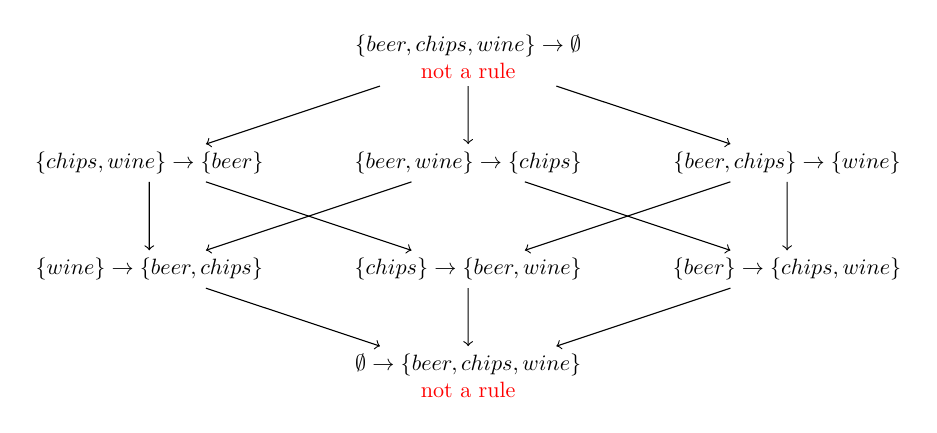
\begin{tikzpicture}[
		scale=0.225,
		every node/.style={scale=0.8}
	]
		
		\node[align=center] (A) at (0,0) {$\{ beer, chips, wine \} \rightarrow \emptyset$ \\ \textcolor{red}{not a rule}};
	
		\node (B) at (-18,-6) {$\{ chips, wine \} \rightarrow \{ beer \}$};
		\node (C) at (0,-6) {$\{ beer, wine \} \rightarrow \{ chips \}$};
		\node (D) at (18,-6) {$\{ beer, chips \} \rightarrow \{ wine \}$};
	
		\node (E) at (-18,-12) {$\{ wine \} \rightarrow \{ beer, chips \}$};
		\node (F) at (0,-12) {$\{ chips \} \rightarrow \{ beer, wine \}$};
		\node (G) at (18,-12) {$\{ beer \} \rightarrow \{ chips, wine \}$};
	
		\node[align=center] (H) at (0,-18) {$\emptyset \rightarrow \{ beer, chips, wine \}$\\ \textcolor{red}{not a rule}};
	
		\draw[->] (A) -- (B);
		\draw[->] (A) -- (C);
		\draw[->] (A) -- (D);
	
		\draw[->] (B) -- (E);
		\draw[->] (B) -- (F);
		\draw[->] (C) -- (E);
		\draw[->] (C) -- (G);
		\draw[->] (D) -- (F);
		\draw[->] (D) -- (G);
	
		\draw[->] (E) -- (H);
		\draw[->] (F) -- (H);
		\draw[->] (G) -- (H);
	
	\end{tikzpicture}
\end{figure}